Imagine a mobile vending machine $VM$ connected by wireless link $talk$ to a shop $Shop1$. On signal fading the $Shop1$ decides to send the link $talk$ to another shop $Shop2$ through the link $switch$ as shown in \refFig{fig_oz_mobile_vending_machine_and_shops}. \oz{} can be used to model the shop. But, the operation $switch$ has a dual nature. It plays the sender role in $Shop1$, and the receiver role in $Shop2$.
 In \oz{} to deal with this duality nature we introduce the concept of \findex{Operation schema overloading}. As in some programming languages, method overloading is the ability to create multiple methods of the same name with different implementations. That is, the operation $switch$ has two different specifications ,i.e. two operation schemas with the same name as shown in \refFig{fig_oz_overloaded_operation_shop}, the first for sending the link $talk$ and the second for receiving it.
\begin{figure}[H]%
\centering
\subcaptionbox{Before switch}{\fbox{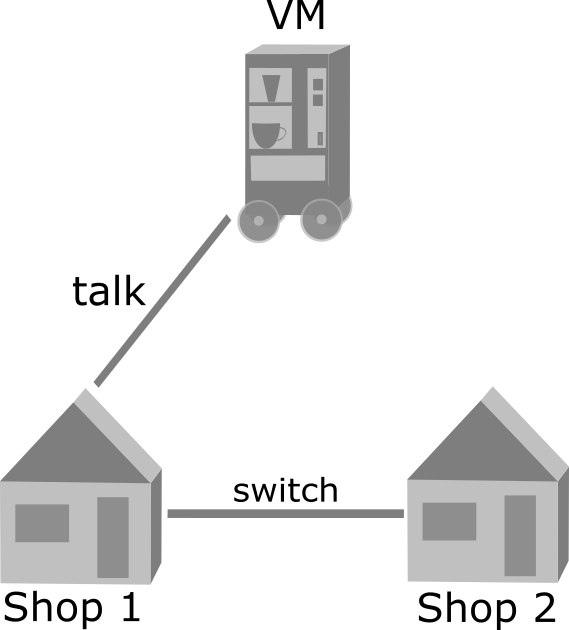
\includegraphics[width=0.45\textwidth]{./images/preliminaries/oz/oz_mobile_vending_machine_and_shops1.png}}}%
\hfill
\subcaptionbox{After switch}{\fbox{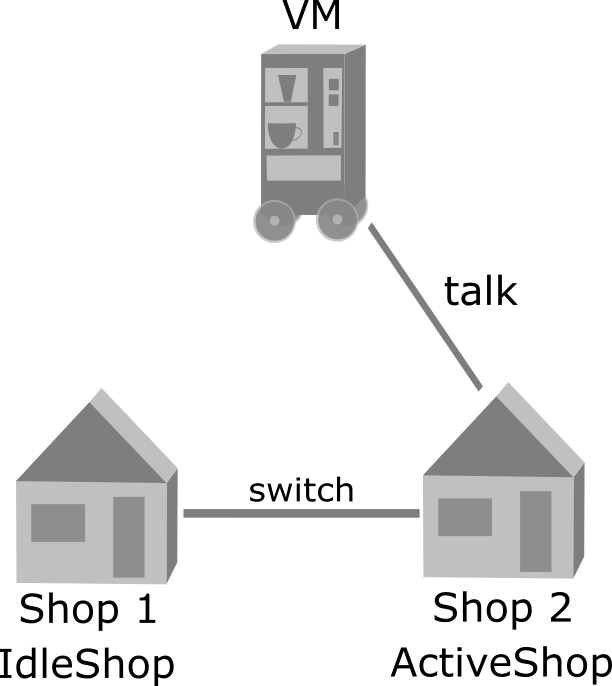
\includegraphics[width=0.45\textwidth]{./images/preliminaries/oz/oz_mobile_vending_machine_and_shops2.png}}}%
\caption{Mobile vending machine and shops}
\label{fig_oz_mobile_vending_machine_and_shops}%
\end{figure}

\begin{figure}[H]
\centering
\begin{class}{Shop(id: \integer)}
\\
\begin{state}
m, vmId, self: \integer
\end{state} 
\\
\begin{init}
\\self = id
\end{init} 
\\
\begin{op}{switch}
x!: chan[\integer \times \integer]
\ST
x! = talk
\end{op}
\\
\begin{op}{switch}
\\x?: chan[\integer \times \integer]
\ST
x? = talk
\end{op}
\\
\begin{op}{talk}
\Delta (m,vmId)
\\y?: \integer
\\z?: \integer
\ST
y? = m'
\\z? = vmId'
\end{op}
\end{class}
\caption{$Shop$ class: \textit{operation schema overloading.}}
\label{fig_oz_overloaded_operation_shop}
\end{figure}

